
%\documentclass[useAMS, usenatbib, fleqn]{mn2e}

% PRD specific
\documentclass[aps,prd,showpacs,superscriptaddress,groupedaddress]{revtex4}  % twocolumn submission
%\documentclass[aps,preprint,showpacs,superscriptaddress,groupedaddress]{revtex4}  % for double-spaced preprint
\usepackage{dcolumn} % needed for some tables
\usepackage{bm}  % for math
% avoids incorrect hyphenation, added Nov/08 by SSR
\hyphenation{ALPGEN}
\hyphenation{EVTGEN}
\hyphenation{PYTHIA}

\usepackage{microtype}
\usepackage{aas_macros}
\usepackage{times}
%\usepackage{txfonts}
\usepackage{url}
\usepackage{amsmath}
\usepackage{amsbsy}
\usepackage{graphicx}
\usepackage{subfig}
\usepackage{xspace}
\usepackage{float}
\usepackage{caption}
\usepackage{amsfonts}
\usepackage{amssymb}
\usepackage{multirow}
\usepackage{color}	
\usepackage[breaklinks, colorlinks, citecolor=blue, linkcolor=black, urlcolor=black]{hyperref}%with colors
%\usepackage{hyperref}%without colors



\newcommand{\ie}{{{i.e.}~}}
\newcommand{\eg}{{{e.g.}~}}
\newcommand{\equref}[1]{{\xspace}Eq.~(\ref{#1})}
\newcommand{\figref}[1]{{\xspace}Fig.~\ref{#1}}
\newcommand{\equrefbegin}[1]{{\xspace}Equation~(\ref{#1})}
\newcommand{\figrefbegin}[1]{{\xspace}Figure~\ref{#1}}
\newcommand{\secref}[1]{{\xspace}Sec.~\ref{#1}}
\renewcommand{\d}{{\mathrm{d}}}
\newcommand{\equ}[1]{\begin{equation}#1\end{equation}}
\newcommand{\eqn}[1]{\begin{eqnarray}#1\end{eqnarray}}
\renewcommand{\vec}[1]{\bmath{#1}}
\newcommand{\negsp}[1]{\hspace*{-#1mm}}

\newcommand{\gal}{g}
\newcommand{\nobj}{{N_{\rm stars}}}
\newcommand{\band}{b}

\newcommand{\todo}[1]{\textcolor{blue}{[TODO: #1]}}
\newcommand{\bl}[1]{\textcolor{blue}{[BL: #1]}}
\newcommand{\dwh}[1]{\textcolor{cyan}{[DWH: #1]}}

\sloppy\sloppypar\raggedbottom\frenchspacing
\begin{document}

 
\title{Shrinking stellar parallax uncertainties with color-magnitude information \\
  but no use of physical stellar models}

\author{Boris~Leistedt}
  \email{boris.leistedt@nyu.edu}
  \affiliation{Center for Cosmology and Particle Physics, Department of Physics, New York University, 726 Broadway, New York, NY 10003, USA}
  \affiliation{NASA Einstein Fellow}
  
\author{Andrew~R.~Casey}
  \affiliation{Institute  of  Astronomy, University  of  Cambridge, Mad-ingley Road, Cambdridge, CB3 0HA, United Kingdom}
 
\author{David~W.~Hogg}
  \affiliation{Center for Cosmology and Particle Physics, Department of Physics, New York University, 726 Broadway, New York, NY 10003, USA}
  \affiliation{Center for Data Science, New York University, 60 Fifth Avenue, New York, NY 10011, USA}
  \affiliation{Flatiron Institute, 162 Fifth Avenue, New York, NY 10010, USA}
  
\begin{abstract}
We present a hierarchical probabilistic model for improving parallax-based stellar distances estimates using color--magnitude information. 
This is achieved with a data driven model of the color--magnitude diagram, not relying on stellar models but instead on the  relative abundances of stars in color--magnitude cells.
The latter are inferred from noisy magnitudes and parallaxes using an efficient sampling method, which is equivalent to deconvolving observational errors into a probabilistic noiseless color--magnitude diagram.
While the latter can be useful for a range of applications, we focus on leveraging multicolor information to provide more accurate stellar distance estimates.
We demonstrate the power of this approach on the Gaia TGAS data sample cross-matched with APASS magnitudes.
As expected, the improvement is more pronounced in the dense regions of the color--magnitude diagram.
We find that the number of objects with signal-to-noise ratio lower than 20 is halved, and that the distance errors are also halved for 20\% of objects.
We make our improved distance estimates publicly available.
\end{abstract}

\pacs{TODO}

\maketitle

  
%%%%%%%%%%%%%%%%%%%%%%%%%%%%%%%%%%%%%%
\section{Introduction}


%%%%%%%%%%%%%%%%%%%%%%%%%%%%%%%%%%%%%%
\section{Model}


\begin{table} %%%%
\centering
\begin{tabular}{cl}
\hline
$s$	&	index of object (the $s$-th star)\\
$d_s, \varpi_s, M_s, C_s$	&	true distance, parallax, absolute magnitude, and color	\\
$\hat{\varpi}_s, \sigma_{\hat{\varpi}_s}^2$ 	&	parallax estimate and its variance\\
$\hat{m}_s, \hat{C}_s, \sigma^2_{\hat{m}_s}, \sigma^2_{\hat{C}_s}$ 	&	apparent magnitude and color estimates, and their variances\\
$b_s$	&	index of the color--magnitude bin of the $s$th object\\
\hline
$b$	&	generic index of color--magnitude bin\\
$n_b$	& 	object count in the $b$-th color--magnitude bin  \\
$\{n_b\}$	&	set of all galaxy counts $n_b$, summing to $\nobj$\\
$f_b$	&	fractional galaxy count in the $b$-th color--magnitude bin  \\
$\{f_b\}$	&	set of all fractional bin counts $f_b$, summing to $1$\\
$\{ d_s, b_s\}$	&	set of properties of all stars in the sample	\\
$\{ \hat{m}_s, \hat{C}_s \}$ &	\\
$\{ d_s, b_s, \hat{m}_s, \hat{C}_s, \hat{\varpi}_s \}$	 	&	\\
\hline
\end{tabular}
\caption{Summary of our notation. }
\label{tab:notation}
\end{table} 

We consider a set of stars indexed as $s=1, \cdots, \nobj$, each characterized by a distance $d_s$, an absolute magnitude $M_s$, and a color $C_s$. 
The magnitude and color are taken with respect to an arbitrarily chosen reference band.
We only consider one color for simplicity, but it should be noted that the models and methods presented below are straightforwardly extended to multiple colors.

The distance to each source is probed by its parallax $\varpi_s=1/d_s$, for which we have an estimate $\hat{\varpi}_s$ with a known Gaussian variance $\sigma_{\hat{\varpi}_s}^2$.
The absolute magnitude and color are not known either: we only have a set of apparent magnitude measurements at our disposal. 
Here, we will consider two magnitudes only, $\hat{m}_s$ and $\hat{m}^\prime_s$, assumed to be  uncorrelated and have Gaussian variances $\sigma_{\hat{m}_s}^2$ and $\sigma_{\hat{m}^\prime_s}^2$.
We will use the first one $\hat{m}_s$ as a reference magnitude for infer the absolute magnitude $M_s$, and the second one to form a color estimate $\hat{C}_s =\hat{m}^\prime_s - \hat{m}_s $ with Gaussian variance $\sigma_{\hat{C}_s}^2 = \sigma_{\hat{m}_s}^2 + \sigma_{\hat{m}^\prime_s}^2$.

In this work, we aim at estimating the distance $d_s$ of each star from the noisy data $\hat{m}_s$,  $\hat{C}_s$ and $\hat{\varpi}_s$. 
While distance is obviously probed by the parallax, it is also informed by the apparent magnitude since $m_s = M_s + 5\log_{10} d_s$ where $d_s$ is expressed in units of $10$ pc.
However, given the apparent magnitude, distance and absolute magnitude are degenerate and cannot be disentangled. 
This degeneracy is partially broken when parallax information is available.
In this work we aim to go even further, and incorporate the knowledge that stars do not have arbitrary colors and magnitude.
In other words, we want to incorporate a prior information $p(M_s, C_s)$ for each star, in order to improve the parallax-based distance estimate. 

\eqn{
	p(d_s | \hat{m}_s, \hat{C}_s, \hat{\varpi}_s, \{ f_{b} \}) = \int \d M_s \ \d C_s \ p\bigl(\hat{m}_s, \hat{C}_s, \hat{\varpi}_s \bigr\rvert M_s, d_s, C_s\bigr) \ p\bigl( M_s, d_s, C_s | \{ f_{b} \} \bigr) \label{eq:distposterior}
}
This integral marginalizes over the true absolute magnitude and color, which might be expensive to perform numerically. 
However, the choices we will make below will allow us to perform it analytically.

The first term of \equref{eq:distposterior} is a likelihood function, and the second term is the prior. 
Assuming that the magnitude and parallax estimates are independent, the likelihood factorizes as the product of two terms, 
\equ{
	p\left(\hat{\varpi}_s \bigr\rvert d_s\right) = \mathcal{N}\bigl(\hat{\varpi}_s - d_s^{-1};\sigma_{\hat{\varpi}_s}^2 \bigr),
}
and
\equ{
	p\bigl(\hat{m}_s, \hat{C}_s \bigr\rvert M_s, d_s, C_s\bigr)  =  \mathcal{N}\bigl( M_s + 5\log_{10}d_s  -\hat{m}_s ;\sigma_{\hat{m}_s}^2 \bigr) \  \mathcal{N}\bigl(\hat{C}_s - C_s;\sigma_{\hat{C}_s}^2 \bigr).
}


In \equref{eq:distposterior}, we have introduced $\{ f_{b} \}$ to parametrize the prior. 
The is a number of possibilities for positing and exploiting this parameterization.
In this work, we construct a model of the relative abundance of objects in color--magnitude cells (two dimensions: absolute magnitude and color) and drop the distance dependency.
In other words, we use a uniform prior for the distance, in order to focus on including multicolor information.
We describe the color--magnitude prior as a linear mixture of $B$ components,
\equ{
	p\left(M_s, C_s  \bigr\rvert \{ f_{b} \} \right) = \sum_{b=1}^B f_b K_b(M_s, C_s),
} 
with $K_b$ the kernel of the $b$th component. 
In other words, the parameters $\{ f_{b} \}$ refer to the relative probabilities of finding objects in the various cells, and must sum to one ($\sum_b f_b = 1$).

While the kernels can be arbitrarily chosen, we adopt Gaussian distributions to make the integral of \equref{eq:distposterior} analytically tractable.
The $b$-th cell is a Gaussian centered at $(\mu_{b,0}, \mu_{b,1})$  with diagonal covariance $(\sigma_{b,0}^2, \sigma_{b,1}^2)$.
We take $\mu_{b+1,0}-\mu_{b,0} = \sigma_{b,0}$ and $\sigma_{b,0}$ constant (similary for the other dimension) to uniformly and contiguously tile a rectangular region of interest of the color--magnitude space with maximum flexibility. 
With this parameterization, the integral of \equref{eq:distposterior} is tractable and leads to
\equ{
	p(d_s | \hat{m}_s, \hat{C}_s, \hat{\varpi}_s, \{ f_{b} \}) \propto f_b \ \mathcal{N}\bigl(\hat{\varpi}_s - d_s^{-1};\sigma_{\hat{\varpi}_s}^2 \bigr) \  \mathcal{N}\bigl( \mu_{b_s,0} + 5\log_{10}d_s  -\hat{m}_s ;\sigma_{\hat{m}_s}^2 + \sigma_{b_s,0}^2 \bigr) \  \mathcal{N}\bigl(\hat{C}_s - \mu_{b_s,1};\sigma_{\hat{C}_s}^2 + \sigma_{b_s,1}^2 \bigr).
}

Finally, to facilitate the parameter inference, we will introduce a latent variable $b_s$ denoting the bin the $s$ object belongs to.
Then, we can equivalently write
\eqn{
	p\left(b_s \bigr\rvert \bigl\{ f_b \bigr\}\right) &=& f_{b_s} \\ 
	p\left(M_s, C_s \bigr\rvert b_s \right) &=& \mathcal{N}\bigl(M_s - \mu_{b,0};\sigma_{b,0}^2 \bigr)  \ \mathcal{N}\bigl(C_s - \mu_{b,1};\sigma_{b,1}^2 \bigr).
}
Our notation is summarized in Table~\ref{tab:notation}.


%%%%%%%%%%%%%%%%%%%%%%%%%%%%%%%%%%%%%%
\subsection{Inference}

Assuming that the bin locations and covariances are fixed, our color--magnitude model is fully described by the relative probabilities $\{ f_{b} \}$. 
If they are fixed by prior knowledge (\eg, external data or stellar models), then one can use \equref{eq:distposterior} to infer the distance of each object using both parallax and color--magnitude information.
Here, we seek to infer $\{ f_{b} \}$ too.
Thus, the full posterior of interest is $p(\{ d_s \}, \{ f_{b} \} | \{ \hat{m}_s, \hat{C}_s, \hat{\varpi}_s \})$, which has $B + \nobj$ parameters.

Given the number of parameters and the natural degeneracies between magnitudes and distances, standard sampling techniques may be difficult to apply.
Thus, we develop a Gibbs sampling strategy, to draw samples from $p(\{ f_{b} \},\{d_s, b_s\}  \rvert \{\hat{m}_s, \hat{C}_s, \hat{\varpi}_s\})$, including the bins $\{ b_s\}$ since it will simplify the inference. 
At the $i$th iteration, we will draw new values of the $\{ f_{b} \}$ and $\{d_s, b_s\}$ parameters given the parameters from the previous iteration, in the following order (the conditional distribution will be made explicit below):
First, draw $\{ f_{b} \}^{(i)}$ given $\{d_s, b_s\}^{(i-1)}$ and the data. 
Second, for each object draw $b_s^{(i)}$ given $\{ f_{b} \}^{(i)}$ and $\{d_s\}^{(i-1)}$ and the data. 
Finally, for each object draw $d_s^{(i)}$ given $\{ f_{b} \}^{(i)}$ and $\{b_s\}^{(i)}$ and the data.
The sequence $\{ f_{b} \}^{(i)},\{d_s, b_s\}^{(i)}$ for $i=1, \cdots, N_\mathrm{samples}$ forms a Markov Chain with the target posterior distribution of interest as equilibrium distribution.
This allows us to avoid the magnitude--distance degeneracies and parallelize the second and third steps over objects.
We know detail how to draw from the correct conditional distributions.

The first draw is standard: with the bin locations $\{b_s\}$ fixed, the fractional weights $\{ f_{b} \}$ follow a Dirichlet distribution entirely determined by $\{n_b \}$, with $n_b$ the number of objects in the $b$-th bin.
All the other parameters enter the constant proportionality factor, so the target distribution is
\eqn{
	p\left(\bigl\{ f_b \bigr\} \bigr\rvert \bigl\{ d_s, b_s, \hat{m}_s, \hat{C}_s, \hat{\varpi}_s \bigr\} \right) \propto p\bigl( \bigl\{ f_b \bigr\} \bigr\rvert \{n_b \} \bigr) \propto \prod_b \frac{ f_b^{n_b} }{n_b !}
}
which can be sampled from using standard techniques for Dirichlet draws.
This first step is the only part involving all objects. The two other steps, \ie drawing $\{d_s, b_s\}$, can be performed for each object independently (and in parallel).

Drawing the bins $b_s$ is also simple, since those are discrete and with the other parameters kept fixed they follow a multinomial distribution with fractional weights given by
\eqn{
	p\left(b_s \bigr\rvert \bigl\{ f_b \bigr\}, d_s, \hat{m}_s, \hat{C}_s, \hat{\varpi}_s\right) &\propto& f_{b_s} \  \mathcal{N}\bigl( \mu_{b_s,0} + 5\log_{10}d_s  -\hat{m}_s ;\sigma_{\hat{m}_s}^2 + \sigma_{b_s,0}^2 \bigr) \  \mathcal{N}\bigl(\hat{C}_s - \mu_{b_s,1};\sigma_{\hat{C}_s}^2 + \sigma_{b_s,1}^2 \bigr).
}

The final step is more complex since the target probability of $d_s$ given the other parameters,
\eqn{
	p\left(d_s \bigr\rvert \bigl\{ f_b \bigr\}, b_s, \hat{m}_s, \hat{C}_s, \hat{\varpi}_s\right) &\propto&  \mathcal{N}\bigl(\hat{\varpi}_s - d_s^{-1};\sigma_{\hat{\varpi}_s}^2 \bigr) \  \mathcal{N}\bigl( \mu_{b,0} + 5\log_{10}d_s  -\hat{m}_s ;\sigma_{\hat{m}_s}^2 + \sigma_{b,0}^2 \bigr) ,\label{eq:distmargposterior}
}
does not follow a simple analytic law.
However, it is simple enough that it could be gridded and drawn from manually, using an inverse transform method, for example.
Here, we adopt an even more direct method: given that this expression admits trivial gradients and is visibly unimodal, we can use Hamiltonian Monte Carlo, and sample from \equref{eq:distmargposterior}. 
We dynamically adjust the stepsize to optimize the exploration of this distribution.


%%%%%%%%%%%%%%%%%%%%%%%%%%%%%%%%%%%%%%
\subsection{Discussion}

Technical advantages and drawbacks of our model

Flexibility of tiling, resolution, and kernel shape (covariance) not affecting the technology

HMC requires differentiable functions. Essential for parameter move with M, log d, m space

Strategy: use large number of noisy parallaxes and colors to infer fb and distances.
Then apply this prior as model to other data via gridding.

%%%%%%%%%%%%%%%%%%%%%%%%%%%%%%%%%%%%%%
\section{Application to TGAS}

We consider the Gaia TGAS sample. We restrict our attention to the objects with valid APASS B and V band magnitudes. 
This significantly reduces the number of objects but allows us to have magnitude, color, and parallax information for X objects. 
We don't apply parallax signal-to-noise (SNR) or color cuts since the purpose of our method is exactly to construct a color magnitude model with both low and high SNR objects. 

We will create a validation sample by randomly extracting X percent of the objects. As detailed below, we will add significant amount of parallax noise and verify that our framework improves the distance estimates consistently with the original estimates. 
We also split the main sample into equal parts with the best and worst parallax SNR, respectively. We perform the inference on the three samples. 

For each of the three samples, we draw 1000 samples of the fractional bin weights, bins, and distances using the Gibbs sampler presented above. 

On figure X we show the color magnitude diagrams obtained with the mean and standard deviation of the fractional bin weights. 
Note that the bins are correlated due to the size of the errors in the individual objects. 
We also show the incorrect color magnitude diagrams obtained by making a histogram of the color and magnitude point estimates (...). 
As expected, the recovered models are narrowed since we are effectively deconvolving observational errors to produce a noiseless color magnitude diagram. 
The red giant branch is successfully recovered too. 
Figure X shows the results on the subsamples obtained with parallax SNR cuts. Those demonstrate that including the noisiest objects is essential for inferring the fainter regions of magnitude space. 

Simplify key figure : show noisy data (with errors?), HR diagram and errors (1x3). Separately show split results (2x3).

We compute the mean and standard deviation of the distance samples. We also compute mean and standard deviation for samples of the parallax likelihood. Note that the posterior distributions on distances are not Gaussian, as expected and also shown below, but the standard deviation nevertheless provides a useful metric. 

We now turn to the validation sample. Since we don't have true distances for those objects either, we take a different approach : we add noise to the parallax estimate, and a level equal to ten times the actual parallax error. We then compute the posterior distribution on the distance (on a distance grid) using the parallax likelihood of eqX as well as the distance posterior of EQX. We simply use the mean model shown in figure X for the color-magnitude prior. 

Show distance results for training, to demonstrate that the HmC works. 


\begin{figure}
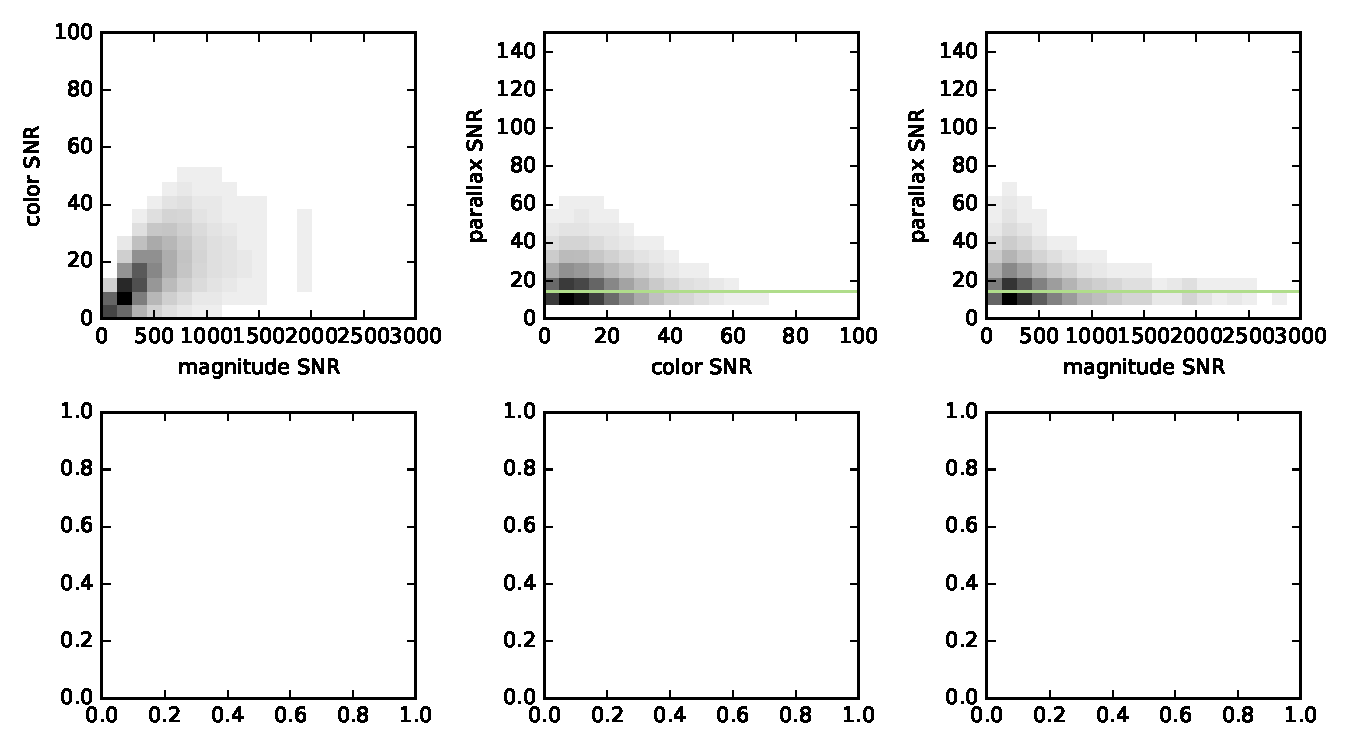
\includegraphics[width=17cm]{datasummary.pdf}
\caption{DATA: colors vs magnitudes vs parallaxes vs errorsParallax and color errors for training and validation sets}
\end{figure}

\begin{figure}
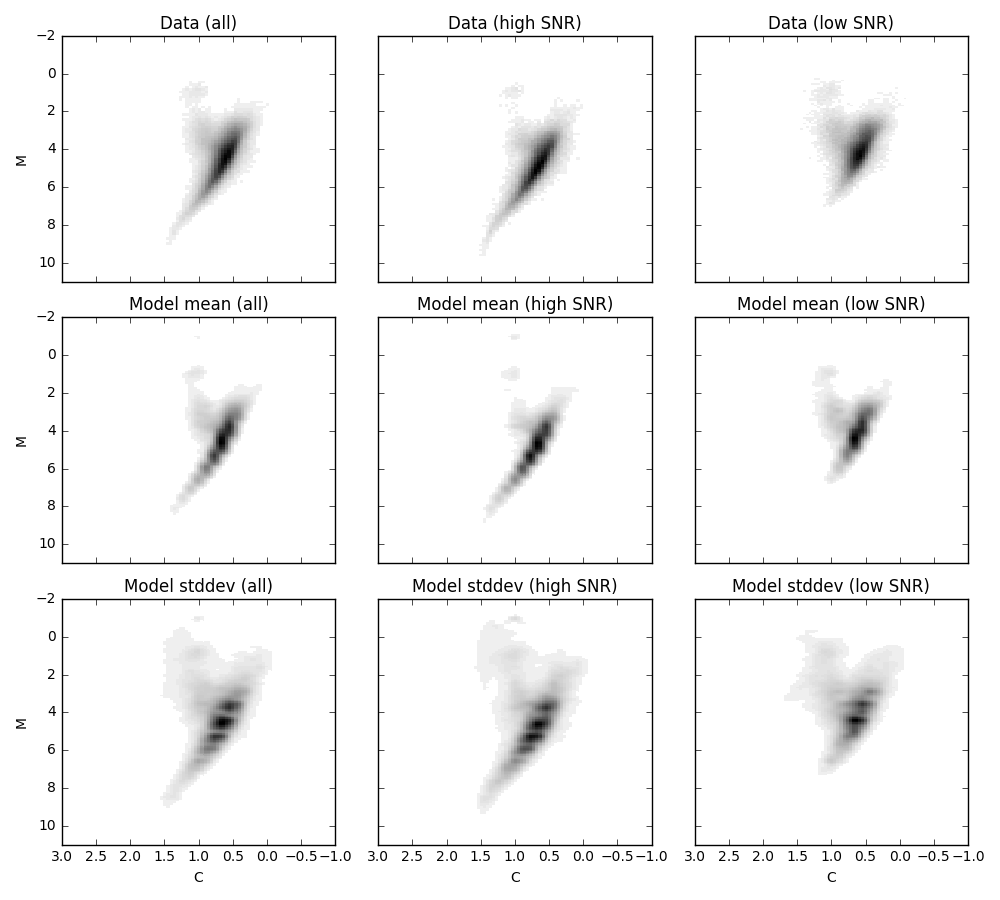
\includegraphics[width=17cm]{colmagdiag_threemeanstd.png}
\caption{3 deconvolved HRD with error maps. 3 Noisy HRD with errors or not? }
\end{figure}

\begin{figure}
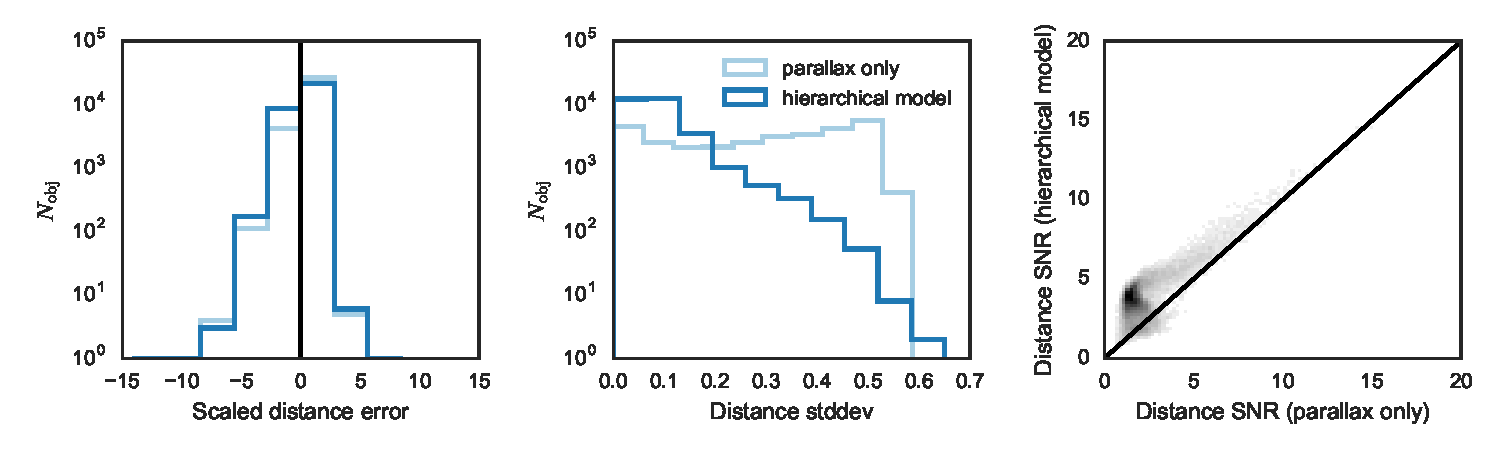
\includegraphics[width=17cm]{metrics.pdf}
\caption{Validation distances : scatter plot of distances without and with shrinkage}
\end{figure}

\begin{figure}
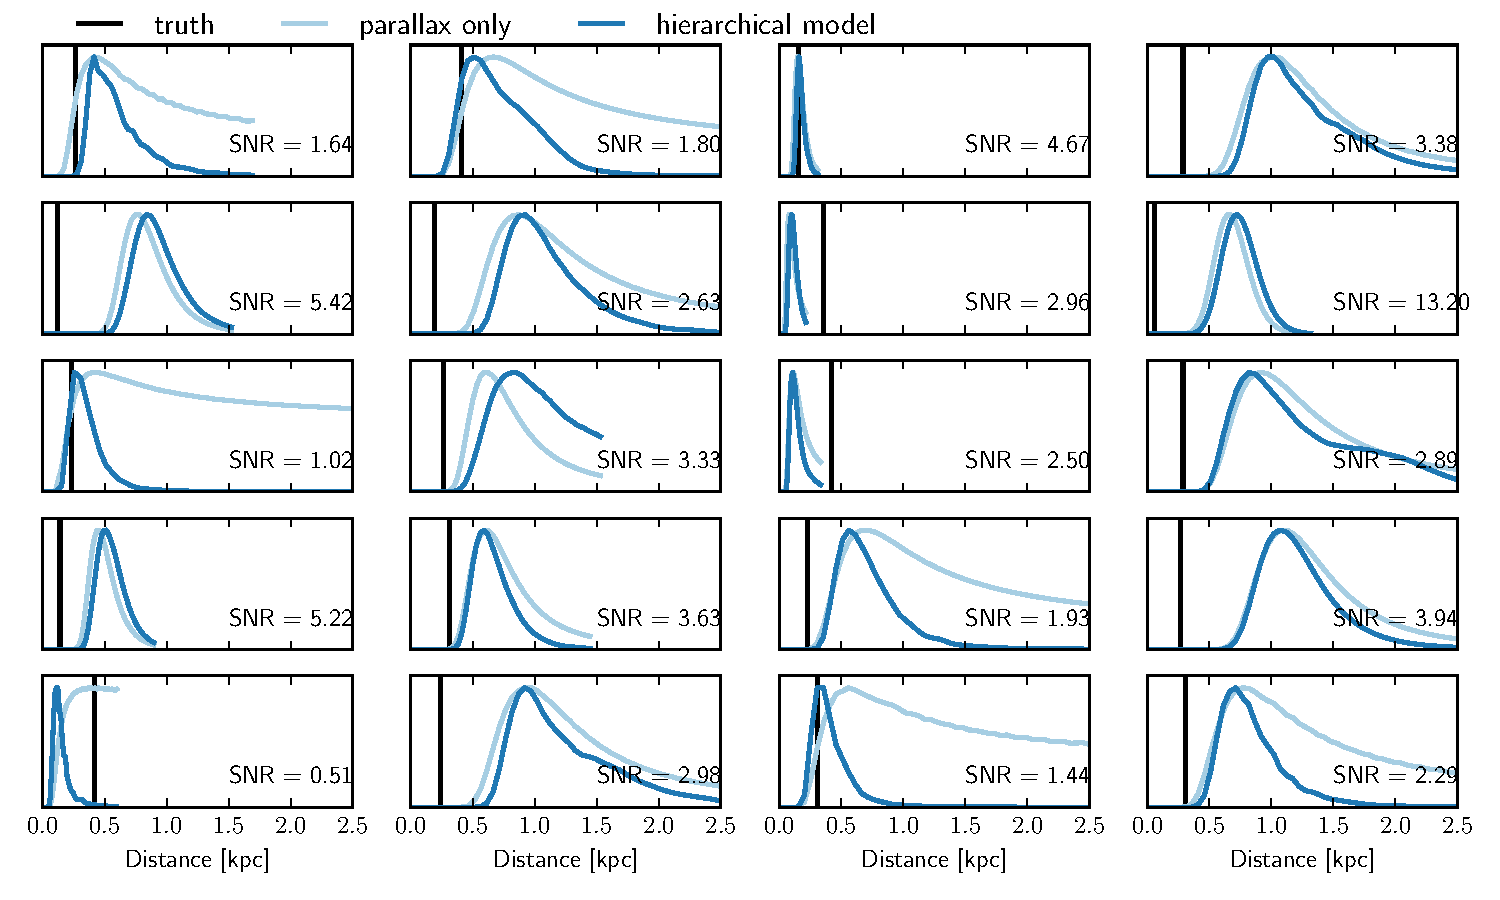
\includegraphics[width=17cm]{cv_noisified_pdfs.pdf}
\caption{Show a few PDFs, including some with basically no parallax measurements}
\end{figure}


\begin{figure}
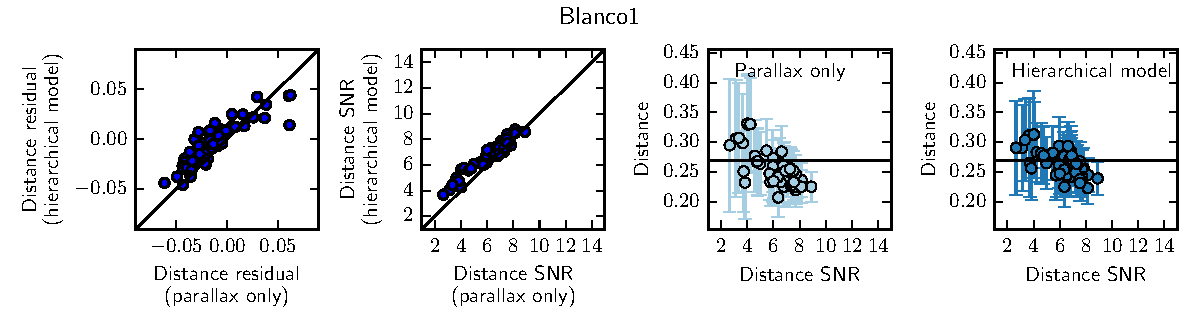
\includegraphics[width=17cm]{Blanco1_metrics.pdf}
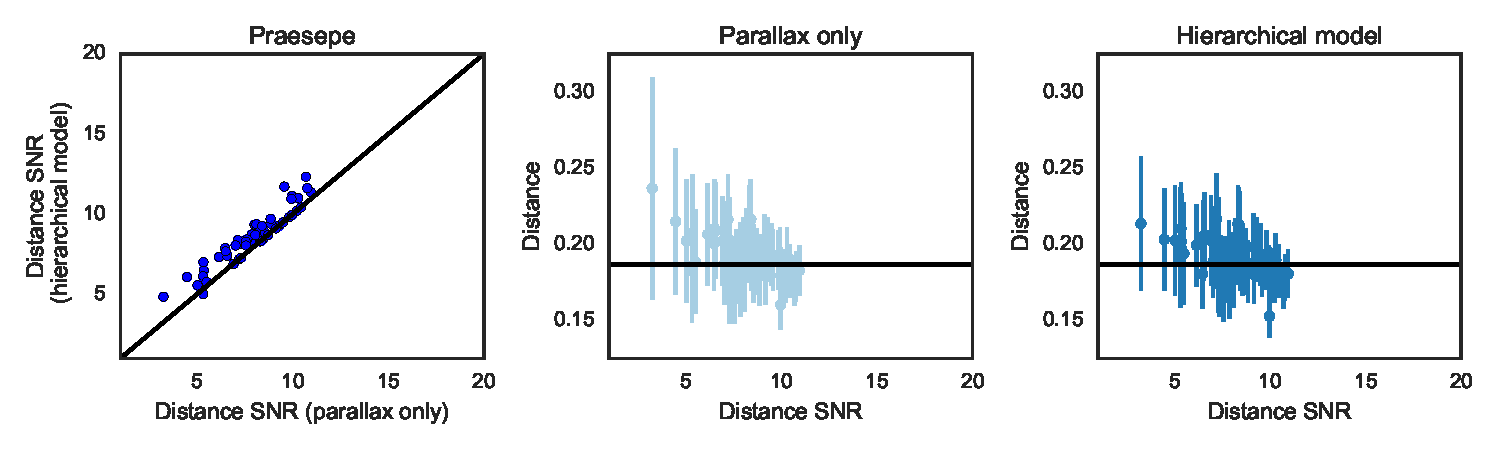
\includegraphics[width=17cm]{Praesepe_metrics.pdf}
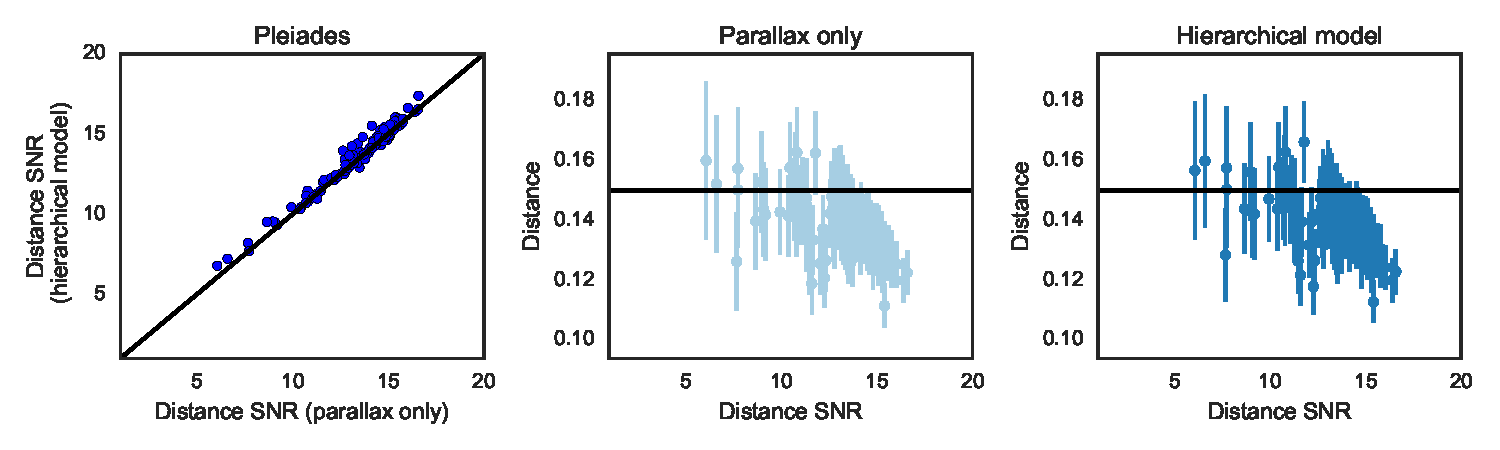
\includegraphics[width=17cm]{Pleiades_metrics.pdf}
\end{figure}


%%%%%%%%%%%%%%%%%%%%%%%%%%%%%%%%%%%%%%
\section{Conclusion}

Could include distance prior



%%%%%%%%%%%%%%%%%%%%%%%%%%%%%%%%%%%%%%
\section{Acknowledgements}

\todo{Add Andy's Acknowledgements}.
BL was supported by NASA through the Einstein Postdoctoral Fellowship (award number PF6-170154).
DWH was partially supported by the NSF (AST-1517237) and the Moore--Sloan Data Science Environment at NYU.

This project was developed in part at the 2016 NYC Gaia Sprint, hosted by the Center for Computational Astrophysics at the Simons Foundation in New York City.

This work has made use of data from the European Space Agency (ESA) mission Gaia (\url{http://www.cosmos.esa.int/gaia}), processed by the Gaia Data Processing and Analysis Consortium (DPAC, \url{http://www.cosmos.esa.int/web/gaia/dpac/consortium}). Funding for the DPAC has been provided by national institutions, in particular the institutions participating in the Gaia Multilateral Agreement.



%%%%%%%%%%%%%%%%%%%%%%%%%%%%%%%%%%%%%%
\bibliography{bib}

%%%%%%%%%%%%%%%%%%%%%%%%%%%%%%%%%%%%%%
\appendix

%% %%%%%%%%%%%%%%%%%%%%%%%%%%%%%%%%%%%%
\end{document}
%% %%%%%%%%%%%%%%%%%%%%%%%%%%%%%%%%%%%%
